\documentclass{article}

\usepackage[brazil]{babel}
\usepackage[T1]{fontenc}
\usepackage[a4paper, left=1.5cm, right=1.5cm, top=2cm, bottom=2cm]{geometry}
\usepackage[colorlinks, urlcolor=blue, citecolor=red]{hyperref}
\usepackage[utf8]{inputenc}
\usepackage[pdftex]{graphicx}
\usepackage{amsfonts, amsmath, enumitem, fancyhdr, float, subcaption}

\pagestyle{fancy}

\fancyhead{}
\fancyfoot[L]{\href{https://github.com/zambonin/ufsc-ine5429}{\texttt{src/}}}
\fancyfoot[C]{\itshape\nouppercase{\leftmark}}
\fancyfoot[R]{\thepage}

\renewcommand{\headrulewidth}{0pt}
\renewcommand{\footrulewidth}{0.75pt}

\fancypagestyle{firststyle} {
    \renewcommand{\headrulewidth}{0.75pt}
    \fancyhead[L]{UFSC -- INE5429}
    \fancyhead[C]{Gustavo Zambonin}
    \fancyhead[R]{\footnotesize{\texttt{gustavo.zambonin@grad.ufsc.br}}}
}

\title{\vspace{-1.5cm}
    \Large{\textbf{
        A função \emph{hash} criptográfica SHA-3
    }}\vspace{-1.5cm}
}
\author{}
\date{}

\begin{document}

\maketitle

\thispagestyle{firststyle}

\section{Definições}

\begin{itemize}

\item Uma \emph{função hash criptográfica}, ou função de resumo criptográfica
(futuramente denotada por $h$), é um algoritmo matemático que mapeia uma
quantidade de bytes qualquer\footnote{algumas funções desse tipo têm
limites quanto ao tamanho da entrada, embora estes sejam extremamente
grandes.} para uma palavra de tamanho fixo, ou seja,
$h : \{0, 1\}^{*} \longrightarrow \{0, 1\}^{n}$, $n \in \mathbb{N}$.

Para que seja resistente a diversos tipos de criptoanálise, uma função
$h : X \longrightarrow Y$ deve respeitar algumas propriedades:

\begin{enumerate}[label=\roman*.]

\item \emph{Resistência à pré-imagem}: Para um resumo $M' \in Y$, é
computacionalmente impraticável\footnote{o tempo ou recursos gastos para esta
computação excedem a validade ou utilidade da informação desejada.} encontrar
a mensagem $M \in X$ tal que $h(M) = M'$. Uma função matemática com esta
propriedade é chamada de unidirecional.

\item \emph{Resistência à segunda pré-imagem}: Para uma mensagem $M_0 \in X$,
é computacionalmente impraticável encontrar uma segunda mensagem $M_1 \in X$
tal que $M_0 \neq M_1$ e $h(M_0) = h(M_1)$.

\item \emph{Resistência à colisão}: Para duas mensagens $M_0, M_1 \in X$, é
computacionalmente impraticável encontrar $M_0 \neq M_1$ e $h(M_0) = h(M_1)$.

\end{enumerate}

É importante notar que, embora as definições sejam extremamente parecidas,
resistência à segunda pré-imagem e resistência à colisão são conceitos
diferentes; um atacante não consegue escolher a primeira mensagem caso queira
atacar a resistência à segunda pré-imagem; para a resistência à colisão, o
atacante pode escolher livremente o par de mensagens.

\item Algumas aplicações destas funções são enumeradas abaixo:

\begin{itemize}

\item Podem ser utilizadas para verificar a integridade da mensagem, comparando
resumos criptográficos calculados antes e depois da transmissão de mensagem
e/ou arquivos.

\item Para evitar o armazenamento de senhas em texto claro, é possível
armazenar apenas o resumo criptográfico de cada senha e compará-lo na
autenticação do usuário.

\item Resumos criptográficos são comumente descritos como identificadores
únicos seguros para um arquivo ou informação digital (por exemplo,
\emph{commits} em um sistema de controle de versão).

\end{itemize}

\item O padrão SHA-3, descrito pelo documento FIPS 202 \cite{Dworkin2015}, é
baseado em uma instância da família \textsc{Keccak} de permutações matemáticas,
selecionada pelo NIST (\emph{National Institute of Standards and Technology})
e especificada neste documento.

\end{itemize}

\section{O algoritmo SHA-3}

\begin{itemize}

\item \textsc{Keccak} é uma família de funções esponja. Este tipo de função é
uma generalização do conceito da função de resumo criptográfica com saída
infinita. Após a aplicação de uma função de preenchimento (\emph{padding}) à
mensagem $M$, a função esponja tem duas fases: a fase de absorção
(\emph{absorbing}), responsável por intercalar blocos de $M$ com aplicações de
uma função de permutação $f$, de modo iterativo; e a fase de compressão
(\emph{squeezing}), onde os blocos de saída, intercalados novamente pela
permutação $f$, são concatenados para gerar uma palavra com um número de bits
configurável pelo usuário. Esse processo pode ser observado na figura
\ref{fig:sponge}.

\item A permutação $f$ é descrita como uma sequência de operações num estado
$A$, que é um vetor de elementos tridimensional em $GF(2)$.
$f$ é uma permutação iterativa, consistindo de uma sequência de rodadas.
Uma rodada $R$ consiste da composição de cinco etapas:
$R = \iota \circ \chi \circ \pi \circ \rho \circ \theta$, como visto
em \ref{fig:steps}:

\begin{enumerate}[label=\roman*.]

\item A etapa $\theta$ faz a soma \texttt{XOR} de um elemento de $A$ e todos
os elementos das colunas adjacentes indicadas.

\item A etapa $\rho$ dispersa os elementos entre cortes transversais verticais
de $A$.

\item A etapa $\pi$ rearranja as posições de elementos em cortes transversais
horizontais de $A$.

\item A etapa $\chi$ tem como efeito fazer a soma \texttt{XOR} de cada bit em
uma linha, de acordo com uma função não-linear de dois outros bits adjacentes.

\item A etapa $\iota$ é utilizada para quebrar a simetria das operações acima,
e sem esta etapa, todas as rodadas teriam a mesma saída. A soma \texttt{XOR} de
alguns bits do estado $A$ é feita com um bit específico de uma sequência gerada
por um LFSR\footnote{\emph{linear-feedback shift register}, um tipo de gerador
de sequências pseudoaleatórias.}, alimentado pelo índice da rodada atual.

\end{enumerate}

\begin{figure}[H]
    \centering
    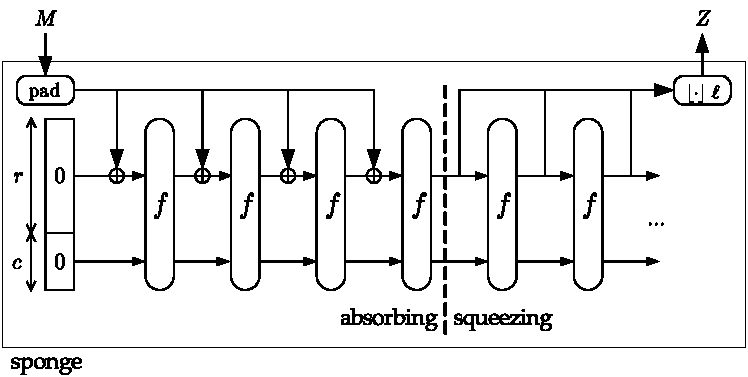
\includegraphics[scale=0.9]{sponge}
    \caption{Uma construção esponja. Imagem retirada de \cite{SpongeReference}.}
    \label{fig:sponge}
\end{figure}

\begin{figure}[H]
    \begin{subfigure}{.5\textwidth}
        \centering
        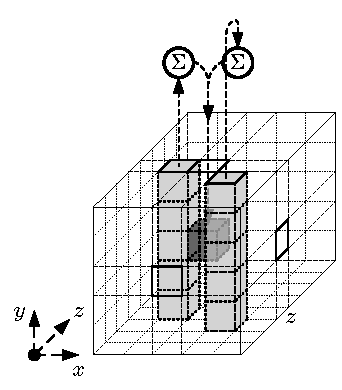
\includegraphics[scale=0.8]{theta_step}
    \end{subfigure}%
    \begin{subfigure}{.5\textwidth}
        \centering
        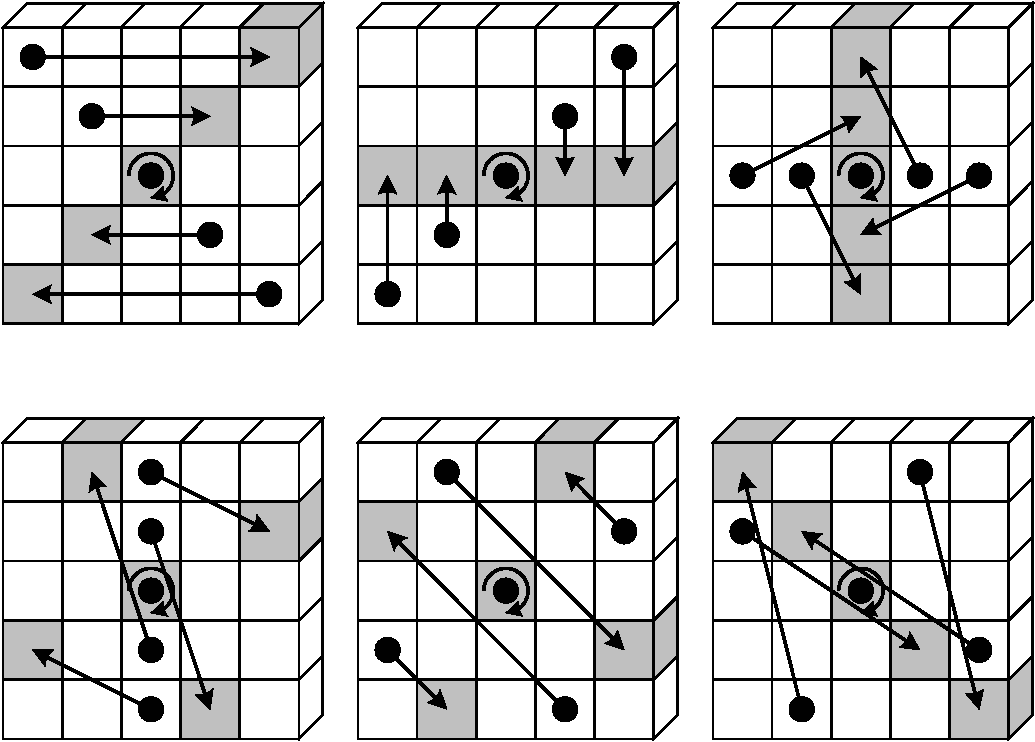
\includegraphics[scale=0.35]{pi_step}
    \end{subfigure}
    \begin{subfigure}{.5\textwidth}
        \centering
        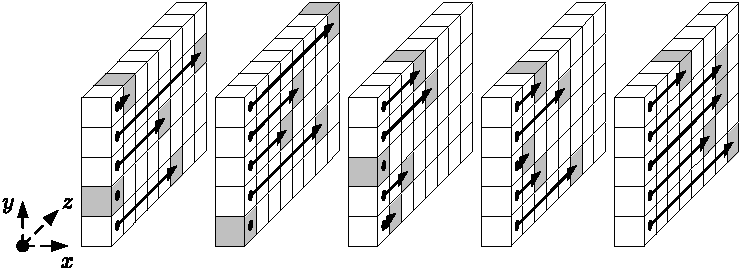
\includegraphics[scale=0.7]{rho_step}
    \end{subfigure}%
    \begin{subfigure}{.5\textwidth}
        \centering
        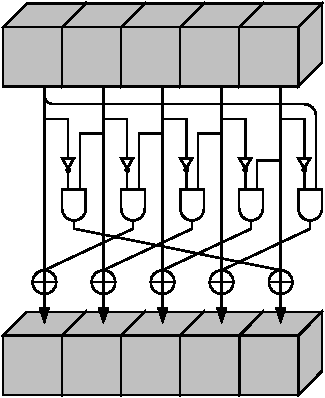
\includegraphics[scale=0.65]{chi_step}
    \end{subfigure}
    \caption{Da esquerda para a direita e de cima para baixo, as etapas
    $\theta$, $\pi$, $\rho$ e $\chi$. Imagens retiradas de
    \cite{KeccakReference}.}
    \label{fig:steps}
\end{figure}

\end{itemize}

\section{Especificações formais}

\begin{enumerate}[label=(\alph*)]

\item O vetor de estados (\emph{state array}) tem como função armazenar
cada estado entre permutações $f$ do \textsc{Keccak}, de modo tridimensional.
Este `'cubo`' tem dimensões $5 \times 5 \times 2^{\ell}$, $\ell \in [0, 6]$, e
$2^{\ell} = w$. O número total de bits neste cubo, denotado por $b$, é
configurável pelo usuário e é geralmente chamado de \emph{largura} do estado;
esta, por sua vez, é dividida em $r + c$ bits, chamados respectivamente de
\emph{taxa} e \emph{capacidade}, como vistos na representação gráfica da
construção esponja (\ref{fig:sponge}).

No vetor de estados, uma raia (\emph{lane}) é um conjunto de $w$ bits onde
apenas a coordenada $z$ muda; um corte transversal vertical (\emph{slice}) é
um conjunto de 25 bits onde apenas a coordenada $z$ é fixa; uma linha é um
conjunto de 5 bits onde apenas a coordenada $x$ muda, e de modo análogo, uma
coluna é um conjunto de 5 bits onde apenas a coordenada $y$ muda.

\item Tome $S$ como uma palavra de $b$ bits que representa um estado na
construção esponja; então, o vetor de estados correspondente é definido como
\begin{align*}
    A[x][y][z] = S[w(5y+x)+z]
    \mid x, y \in \mathbb{Z}_5 \land z \in \mathbb{Z}_w
\end{align*}

Por exemplo, se $b = 200$, então segue que $w = 8$, e portanto:
\begin{align*}
    A[0, 0, 0] &= S[0]   & A[1, 0, 0] &= S[8]  & & \cdots & A[4, 0, 0] &= S[32] \\
    \vdots && \vdots &&& \cdots && \vdots \\
    A[0, 0, 7] &= S[7]   & A[1, 0, 7] &= S[15] & & \cdots & A[4, 0, 7] &= S[39] \\
    A[0, 1, 0] &= S[40]  & A[1, 1, 0] &= S[48] & & \cdots & A[4, 1, 0] &= S[72] \\
    \vdots && \vdots &&& \cdots && \vdots \\
    A[0, 4, 7] &= S[167] & A[1, 4, 7] &= [175] & & \cdots & A[4, 4, 7] &= S[199]
\end{align*}

\item A construção de uma palavra $S$ a partir de um vetor de estados $A$ é
feita pela concatenação ($||$) dos bits de tal modo que $z$ seja incrementado
primeiro, depois $x$, e por fim $y$; a inversa da operação acima.

Por exemplo, se $b = 200$ e $w = 8$:
\begin{align*}
    S = A[0, 0, 0] \mid\mid \cdots \mid\mid A[0, 0, 7] \mid\mid A[1, 0, 0]
    \mid\mid \cdots \mid\mid A[4, 0, 7] \mid\mid A[0, 1, 0] \mid\mid A[0, 1, 1]
    \mid\mid \cdots \mid\mid A[4, 4, 7]
\end{align*}

\item Todas as operações realizadas devem ser sobre módulo 5 nas coordenadas
$x$ e $y$, e módulo $w$ na coordenada $z$. As adições e multiplicações entre
os termos são sobre $GF(2)$, exceto quando notado. Índices omitidos significam
que a operação é válida para todos os valores daquela porção do vetor de
estados.

\begin{itemize}

\item $\theta : A[x][y][z] \longleftarrow A[x][y][z]
    + \displaystyle\sum_{y'=0}^{4} A[x - 1][y'][z]
    + \displaystyle\sum_{y'=0}^{4} A[x + 1][y'][z - 1]$

A etapa $\theta$ foca na difusão de bits no vetor de estados $A$. Sem esta
etapa, a permutação não proveria difusão significativa. Sua utilização leva a
uma maior proteção contra criptoanálise linear e diferencial, além de ataques
algébricos.

\item $\rho : A[x][y][z] \longleftarrow A[x][y][z - (t + 1)(t + 2)/2],
    \begin{pmatrix} 0 & 1 \\ 2 & 3 \end{pmatrix} ^{t}
    \begin{pmatrix} 1 \\ 0 \end{pmatrix}
    = \begin{pmatrix} x \\ y \end{pmatrix} $ em $GF(5)^{2 \times 2}$
    \begin{flushright}
        para $0 \leq t < 24$, ou $t = -1$ se $x = y = 0$.
    \end{flushright}

A etapa $\rho$ consiste de movimentos entre bits de diferentes raias, para
prover uma boa dispersão entre \emph{slices}. Sem esta etapa, esta difusão
seria muito lenta. As novas coordenadas $x_t, y_t$ são definidas através de um
processo iterativo de multiplicação de matrizes.

Tome $M = \begin{pmatrix} 0 & 1 \\ 2 & 3 \end{pmatrix}$ e
$B = \begin{pmatrix} 1 \\ 0 \end{pmatrix}$:
\begin{align*}
    t &= 0 \longrightarrow M^{0} \cdot B
        = \begin{pmatrix} 1 \\ 0 \end{pmatrix} \hspace{1cm}
    t = 1 \longrightarrow M^{1} \cdot B
        = \begin{pmatrix} 0 \\ 2 \end{pmatrix} \\
    t &= 2 \longrightarrow M^{2} \cdot B
        = \begin{pmatrix} 2 \\ 6 \end{pmatrix} \hspace{1cm}
    t = 3 \longrightarrow M^{3} \cdot B
        = \begin{pmatrix} 6 \\ 22 \end{pmatrix}
\end{align*}

Então, pode-se verificar que existe uma relação de recorrência tal que
$(x_{t}, y_{t}) = (y_{t-1}, 2x_{t-1} + 3y_{t-1})$. Estes valores serão
dependentes apenas das dimensões do vetor de estados, então podem ser
pré-computados para que o número de multiplicações entre matrizes seja
reduzido.

\item $\pi : A[x][y] \longleftarrow A[x'][y']$,
    $\begin{pmatrix} x \\ y \end{pmatrix}
    = \begin{pmatrix} 0 & 1 \\ 2 & 3 \end{pmatrix}
    \begin{pmatrix} x' \\ y' \end{pmatrix}$

A etapa $\pi$ é uma transposição das raias, que provê difusão a longo prazo.
Esta etapa mistura bits alinhados horizontalmente e verticalmente de modo que
a criptoanálise diferencial seja dificultada, pois do contrário, suas trilhas
poderiam ser simplificadas, de acordo com \cite{KeccakDC}.

\item $\chi : A[x] \longleftarrow A[x] + (A[x + 1] + 1) \cdot A[x + 2]$

A etapa $\chi$ é a única não-linear, trocando o valor do bit operado se seus
vizinhos forem 0 à esquerda e 1 à direita. Sem esta etapa, a rodada $R$ seria
completamente linear. Pode ser vista como a aplicação paralela de $5 \cdot w$
caixas-S\footnote{\emph{substitution box}, um componente básico de
criptografia simétrica, responsável por mapear uma entrada de tamanho $m$
para uma saída de tamanho $n$ de modo a diluir a relação entre estes. São
cuidadosamente construídas para resistir à criptoanálise linear e diferencial.}
operando em cada linha do vetor de estados.

\item $\iota : A \longleftarrow A + RC[i_r]$, \\
    $RC[i_r][x][y][z] = 0$, \\
    $RC[i_r][0][0][2^j - 1] = rc[j + 7i_r] \; \forall \; 0 \leq j < \ell$, \\
    $rc[t] = (x^t \pmod{x^8 + x^6 + x^5 + x^4 + 1}) \pmod{x}$ em $GF(2)[x]$

A etapa $\iota$ é a única assimétrica, e sem ela, \textsc{Keccak} seria mais
suscetível a ataques que exploram simetria entre rodadas. O vetor $RC[i_r]$
guarda constantes geradas por um LFSR $rc[t]$, e somadas apenas à primeira
linha do vetor de estados. Por conta disso, a perturbação será aumentada nas
etapas $\theta$ e $\chi$ para todas as raias depois de apenas uma rodada.

\end{itemize}

\item A permutação \textsc{Keccak}$-p[b, n_r]$ consiste de $n_r$ iterações
de rodadas $R$ sobre um estado de largura $b$. A permutação
\textsc{Keccak}$-f$, definida em \cite{KeccakReference}, apenas é uma
especialização da família acima, onde o número de rodadas deve ser
correlacionado à profundidade do vetor de estados: $n_r = 12 + 2 \cdot \ell$.
Então, a permutação \textsc{Keccak}$-p[1600, 24]$, que define as seis funções
SHA-3, é equivalente $(\stackrel{\Delta}{=})$ a \textsc{Keccak}$-f[1600]$.
Apenas existe uma diferença na indexação das rodadas das duas permutações.

\item \label{f} Uma construção esponja é um modo de operação, baseado em uma
permutação de tamanho fixo e uma regra de preenchimento (\emph{padding}), que
constrói uma função responsável por mapear uma entrada de tamanho qualquer
para uma saída de tamanho desejável. Tal função é apropriadamente chamada de
\emph{função esponja}, e pode ser reconhecida como uma generalização de
funções de resumo criptográficas, que têm saídas de tamanho fixo, e de cifras
de fluxo (\emph{stream ciphers}), restritas por entradas de tamanho fixo. A
função esponja aplica iterativamente sua permutação interna aos estados
intermediários, construídos por entradas ou saídas anteriores ao estado atual.

A construção aplica sua permutação $f$ sobre estados de $b$ bits. A entrada
$M$ é preenchida de modo que os bits extras, adicionados para tornar o tamanho
dos blocos homogêneo, possam ser retirados ao final do procedimento. Então, é
dividida em blocos de tamanho $r$, denotados $M_r$. Os $b$ bits de cada estado
são inicializados com zero e a construção procede à execução, em duas fases
separadas.

Na fase de absorção (\emph{absorbing}), os blocos $M_r$ são `'\verb!XOR!ados`'
com os primeiros $r$ bits do estado atual, intercalados com aplicações da
permutação $f$. Quando todos os blocos $M_r$ são processados, a esponja passa
para a fase de compressão (\emph{squeezing}), onde os primeiros $r$ bits do
estado são retornados como blocos de saída, também intercalados com aplicações
da permutação $f$. O número de blocos de saída $\ell$ é escolhido pelo usuário,
e a saída $Z$ é truncada de acordo. Os últimos $c$ bits do estado nunca são
diretamente afetados por $M_r$, e também nunca revelados durante a fase de
compressão. Essencialmente, estão correlacionados com o nível de segurança da
esponja.

\item \textsc{Keccak} é a família de funções esponja definidas com a
permutação \textsc{Keccak}$-p[b, 12 + 2\ell]$ junto a uma simples função de
preenchimento \texttt{pad10*1}. Tal função adiciona os bits
$1 \mid\mid 0^{-m-2 \pmod{x}} \mid\mid 1$ à palavra original, onde $m$ é o
resto da divisão inteira do tamanho da palavra pela largura $x$ da esponja.
O asterisco no nome da função significa que é necessário adicionar tantos
`'zeros`' quanto necessário para preencher a palavra de maneira que esta
seja igualmente divisível em blocos.

\item Uma função \textsc{Keccak}$[c](N, d)$ opera sobre uma palavra de bits
de tamanho $N$ e tamanho de saída $d$, com capacidade $c$. Ela pode ser
definida como
\begin{align*}
    \textsc{Keccak}[r, c] &\stackrel{\Delta}{=}
    \textsc{sponge}[\textsc{Keccak}-f[r+c], \texttt{pad10*1}, r](N, d) \\
    \textsc{Keccak}[c] &\stackrel{\Delta}{=} \textsc{Keccak}[r=1600-c, c](N, d)
\end{align*}

e é a base para todas as quatro funções SHA-3. A função \textsc{sponge} é a
representação matemática dos parâmetros explicados acima e será explorada em
\ref{i}.

\begin{enumerate}[label=\roman*.]

\item As quatro funções \emph{hash} SHA-3 recebem uma mensagem $M$ como entrada
e são definidas a partir da função \textsc{Keccak}$[c]$ especificada acima. Em
cada caso, a capacidade é o dobro do tamanho do resumo criptográfico, e todas
as mensagens são sufixadas com a palavra \texttt{01}. Ou seja,
\begin{align*}
    SHA3-224(M) &= \textsc{Keccak}[448](M \mid\mid \texttt{01}, 224) \\
    SHA3-256(M) &= \textsc{Keccak}[512](M \mid\mid \texttt{01}, 256) \\
    SHA3-384(M) &= \textsc{Keccak}[768](M \mid\mid \texttt{01}, 384) \\
    SHA3-512(M) &= \textsc{Keccak}[1024](M \mid\mid \texttt{01}, 512)
\end{align*}

\item Duas outras funções, chamadas de \emph{SHA-3 Extendable-Output Functions}
(SHAKE, ou `'Funções de saída estendida SHA-3`'), são definidas concatenando
\texttt{1111} como sufixo à mensagem $M$. Para qualquer tamanho de saída $d$,
tem-se
\begin{align*}
    SHAKE128(M, d) &= \textsc{Keccak}[256](M \mid\mid \texttt{1111}, d) \\
    SHAKE256(M, d) &= \textsc{Keccak}[512](M \mid\mid \texttt{1111}, d)
\end{align*}

\end{enumerate}

Os bits adicionados como sufixo às mensagens servem para diferenciar entradas
da função \textsc{Keccak}$[c]$ provenientes de SHA-3 ou SHAKE. Esta estratégia
é chamada de separação por domínios (\emph{domain separation}).

\item \label{i} A construção da esponja produz uma função \textsc{sponge}$[f,
\texttt{pad}, r]$, onde $f$ é uma permutação de tamanho fixo, \textsc{pad} é
a função de preenchimento, que adiciona os bits necessários para que a
mensagem seja corretamente dividida em blocos, e $r$ é a taxa de bits da
entrada que passará por dentro da esponja. O estado inicial da esponja é
chamado de estado raiz, e consiste de $0^b$ bits. Uma melhor descrição da
construção pode ser encontrada em \ref{f}.

\item Tradicionalmente, usuários de funções \emph{hash} esperam um nível de
segurança que seja correlacionado com o tamanho da sua saída: $2^{n/2}$ para
resistência à colisão e $2^n$ para resistência à (segunda) pré-imagem, onde
$n$ é o tamanho da saída. Esta característica é respeitada por todas as
funções especificadas pelo NIST. A criptoanálise em instâncias de
\textsc{Keccak}$-f[1600]$ mostra\footnote{como visto em
\url{http://keccak.noekeon.org/Keccak-slides-at-NIST-Feb2013.pdf}} que, ainda
com 8 rodadas, o número de operações necessárias para obter alguma informação
relevante é de $2^{491}$, e $2^{1574}$ para as 24 rodadas propostas no
documento \cite{Dworkin2015}.

\item A convenção para interpretar palavras em base hexadecimal como palavras
de bits, para as entradas e saídas dos algoritmos apresentados, é diferente da
usual: a ordem dos bits para cada byte completo é revertida. Ou seja, se uma
palavra \texttt{0xfb23} deve ser interpretada, então:

\texttt{0xfb23} $\longrightarrow$ \texttt{0b1111101100100011}
$\stackrel{SHA-3}{\longrightarrow}$ \texttt{0b110111111000100}

Exemplos de entradas e saídas de rodadas e etapas intermediárias podem ser
encontrados
\href{http://csrc.nist.gov/groups/ST/toolkit/examples.html#aHashing}
{aqui}, onde as saídas de uma implementação podem ser comparadas a cada passo
para garantir sua acurácia.

\end{enumerate}

\section{Implementação}

\begin{enumerate}[label=(\alph*)]

\item Toda a documentação referente à implementação pode ser encontrada junto
ao próprio código, localizado em \texttt{keccakf1600.py}, no repositório fonte
deste documento. Embora sua performance não seja competitiva, a legibilidade
foi obtida omitindo constantes `'mágicas`' e optando por gerá-las de acordo
com a execução do programa, junto ao funcionamento das outras etapas.

\item A função \texttt{Keccak} contém três partes principais: a absorção, em
157--164; o preenchimento, em 166--170; e a compressão, em 172--178. A
permutação \texttt{keccak\_f\_1600}, por sua vez, abriga as etapas $\theta$ em
103--105, $\rho$ e $\pi$ mescladas em 107--111, $\chi$ em 113--116 e $\iota$ em
118--121. É possível substituir facilmente a etapa assimétrica pelo vetor de
constantes $RC$, e embora trabalhoso, adaptar o código para utilizar o vetor de
constantes $r$ na etapa $\rho$, assim trazendo a implementação mais próxima do
pseudocódigo apresentado em \cite{KeccakImplementation}.

\end{enumerate}

\bibliography{ine5429_t6}
\bibliographystyle{plain}

\end{document}
